\documentclass[a4paper,12pt,handout]{beamer}

%%%%%%%%%%%%%%%%%%%%%%%%%%%%%%%%%%%%%%%%%%%%%%%%%%%%%%%%
% Change to 0 to produce only slides without the notes,%
% to 1 to generate an A4 document with the notes.      %
%%%%%%%%%%%%%%%%%%%%%%%%%%%%%%%%%%%%%%%%%%%%%%%%%%%%%%%%
\def\includeNotes{0}
%%%%%%%%%%%%%%%%%%%%%%%%%%%%%%%%%%%%%%%%%%%%%%%%%%%%%%%%

\usetheme{Pittsburgh}
\usecolortheme{whale}
\usepackage{siunitx}
\usepackage{graphicx}
\graphicspath{{fig/}}

\setbeameroption{hide notes}
\setbeamertemplate{note page}[plain]
\usepackage{pgfpages}

% Define a layout to include 2 slides per page
\makeatletter
\define@key{pgfpagesuselayoutoption}{horizontal shift}%
{\def\pgfpageoptionhshift{#1}}
\define@key{pgfpagesuselayoutoption}{vertical shift}%
{\def\pgfpageoptionvshift{#1}}
\makeatother
\pgfpagesdeclarelayout{2 on 1 shifted}
{
	\edef\pgfpageoptionheight{\the\paperwidth} % landscaped by default
	\edef\pgfpageoptionwidth{\the\paperheight}
	\def\pgfpageoptionborder{0pt}
	\def\pgfpageoptionfirstshipout{1}
	\def\pgfpageoptionhshift{0pt}
	\def\pgfpageoptionvshift{0pt}
}
{
	\pgfpagesphysicalpageoptions
	{%
		logical pages=2,%
		physical height=\pgfpageoptionheight,%
		physical width=\pgfpageoptionwidth,%
		current logical shipout=\pgfpageoptionfirstshipout%
	}
	% stack on top of one another
	\pgfpageslogicalpageoptions{1}
	{%
		border shrink=\pgfpageoptionborder,%
		border code=\pgfusepath{stroke},%
		resized width=\pgfphysicalwidth,%
		resized height=.5\pgfphysicalheight,%
		center=\pgfpoint{.5\pgfphysicalwidth+\pgfpageoptionhshift}%
		{.75\pgfphysicalheight+\pgfpageoptionvshift}%
	}%
	\pgfpageslogicalpageoptions{2}
	{%
		border shrink=\pgfpageoptionborder,%
		resized width=\pgfphysicalwidth,%
		resized height=.5\pgfphysicalheight,%
		center=\pgfpoint{.5\pgfphysicalwidth+\pgfpageoptionhshift}%
		{.25\pgfphysicalheight+\pgfpageoptionvshift}%
	}%
}

\usepackage{ifthen}
\ifthenelse{\equal{\includeNotes}{1}}{%
	\pgfpagesuselayout{2 on 1 shifted}[%
		a4paper,border shrink=10mm, horizontal shift=0cm]
	\setbeameroption{show notes}}{}%


%%%%%%%%%%%%%%%%%%%%%%%%%%%%%%%%%%%%%%%%%%%%%%%%%%%%%%%%%%%

\title{Green communications in 5G}
\author{Tim Van Den Driesschen\\Rodrigo Arias Mallo}
\institute{Universitat Politècnica de Catalunya}
\date{\today}

\begin{document}

\begin{frame}
	\titlepage
\end{frame}
\note{}
%%%%%%%%%%%%%%%%%%%%%%%%%%%%%%%%%%%%%%%%%%%%%%%%%%%%%%%%%%%
\begin{frame}
\frametitle{Introduction}
\begin{itemize}

\item In the next decade, the number of connected devices is expected to 
increase 100 times and the data volume by 1000 times

\item Operators are already facing significant power bills

\item Moving towards green communications is important both for 
\textbf{environmental} and \textbf{economic} reasons

\end{itemize}
\end{frame}
\note{}
%%%%%%%%%%%%%%%%%%%%%%%%%%%%%%%%%%%%%%%%%%%%%%%%%%%%%%%%%%%
\begin{frame}
	\frametitle{Network planning and deployment}
\end{frame}
\note{}
%%%%%%%%%%%%%%%%%%%%%%%%%%%%%%%%%%%%%%%%%%%%%%%%%%%%%%%%%%%
\begin{frame}
\frametitle{Harvesting renewable energy resources}
In order to power the Base Stations (BS), energy can be obtained from renewable 
sources:

\begin{itemize}
\item Natural sources: Sun, wind, vibration
\item External: Batteries, fuel cells
\end{itemize}
\end{frame}
\note{%
Solar energy has been tested to power BS installed in road lamps, with the solar
panel on top [175]. It has been observed that it can run fully autonomous, with
the exception of the January month, where external power was needed.

Other sources of energy may not be so profitable, as sun is the source with the
higest amount of power, about \SI{100}{\milli\watt\per\centi\meter\squared}, 
followed by the wind with \SI{12}{\milli\watt\per\centi\meter\squared}.
}
%%%%%%%%%%%%%%%%%%%%%%%%%%%%%%%%%%%%%%%%%%%%%%%%%%%%%%%%%%%
\begin{frame}
	\frametitle{User-centric designs}
\end{frame}
\note{}
%%%%%%%%%%%%%%%%%%%%%%%%%%%%%%%%%%%%%%%%%%%%%%%%%%%%%%%%%%%
\begin{frame}
	\frametitle{Smaller frame overhead %
		\footnote{Following [178] paper in depth: Uplink Contention Based Multiple 
		Access for 5G Cellular IoT}%
	}

	\begin{itemize}
		\item Bursty traffic cause devices to change state between idle and 
		connected with the associate \textbf{power consumption}
		\item Significant \textbf{overhead} with small packets
		\item Contention based method have been proposed
		\end{itemize}
\end{frame}
\note{Expand based on reference 178}
%%%%%%%%%%%%%%%%%%%%%%%%%%%%%%%%%%%%%%%%%%%%%%%%%%%%%%%%%%%
\begin{frame}
	\frametitle{Uplink contention based methods}


	\begin{center}
	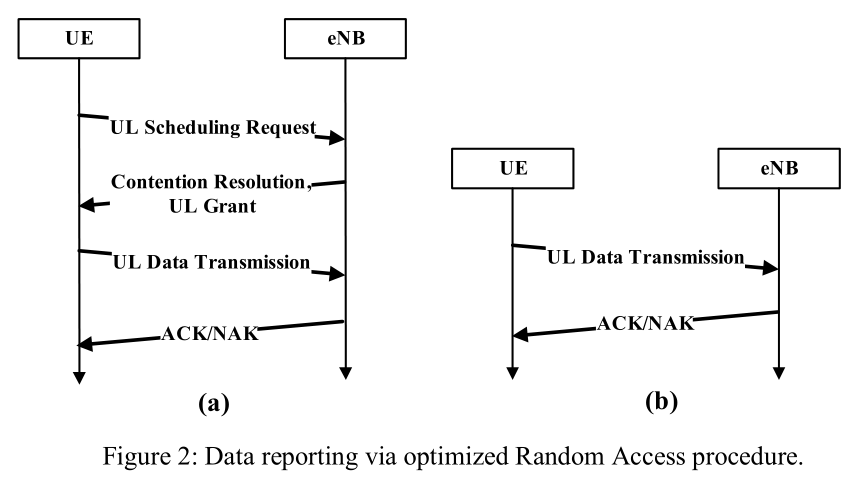
\includegraphics[scale=0.3]{uc.png}
	\end{center}

	\begin{itemize}
		\item Small signalling payload
		\item Direct small data packet
	\end{itemize}
\end{frame}
\note{}
%%%%%%%%%%%%%%%%%%%%%%%%%%%%%%%%%%%%%%%%%%%%%%%%%%%%%%%%%%%
\begin{frame}
	\frametitle{Results of simulation}

	\begin{center}
	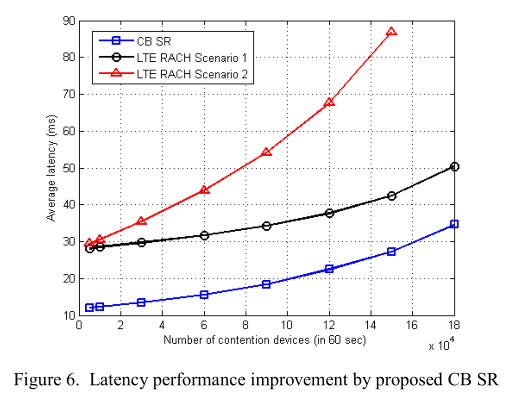
\includegraphics[scale=0.4]{cb-latency.png}
	\end{center}

\end{frame}
\note{}
%%%%%%%%%%%%%%%%%%%%%%%%%%%%%%%%%%%%%%%%%%%%%%%%%%%%%%%%%%%
\begin{frame}
\frametitle{Open problems}

\begin{itemize}
\item Power control in green communications
\item Energy efficient hardware
\item Energy efficient network architecture
\item Battery technology enhancement: sugar bio-batteries %
\footnote{Following [183] paper in depth: \textsl{A high-energy-density sugar 
biobattery based on a synthetic enzymatic pathway}}
\end{itemize}

\end{frame}
\note{}
%%%%%%%%%%%%%%%%%%%%%%%%%%%%%%%%%%%%%%%%%%%%%%%%%%%%%%%%%%%
\begin{frame}
\frametitle{Sugar bio-batteries [183]}

\begin{itemize}

	\item The typical density of energy of a Lithium cell is around 
	\SI{0.54}{\mega\joule\per\kilogram}

	\item But the combustion energy of glucose can release up to 
	\SI{15.5}{\mega\joule\per\kilogram}

	\item Sugars are non toxic, safe and carbon neutral

\end{itemize}
\end{frame}
\note{}
%%%%%%%%%%%%%%%%%%%%%%%%%%%%%%%%%%%%%%%%%%%%%%%%%%%%%%%%%%%
\end{document}

